\section{Visibility between satellites}
\paragraph{}In the following pages we are going to discuss the methodology to obtain the maximum angle between two satellites on the same plane. By doing this, the upper limit of the distance between the satellites will be established. This is necessary to compute some of the constellation parameters. However, this distance is expected to be larger than the maximum distance allowed in order to achieve global coverage

\paragraph{}To compute the angle we have to make some assumptions:
\begin{itemize}
	\item The satellites have antennas pointing to each other.
	\item The atmosphere attenuation is neglected over $113 km$. Below that altitude the signal is fully attenuated.
	\item The antenna have enough power to reach that distance. 
\end{itemize}

\paragraph{}These hypothesis converts the problem into simple geometric calculation because we are neglecting all the physics related to it. Remember that the aim of this code is to obtain a first approach. Nevertheless, the second assumption has an explanation, for frequencies below $3 GHz$ the attenuation caused by clouds, oxigen, and other atmospheric gases can be neglected in the upper layers of the ionosphere (over $113 km$)\cite{Zubair2011}. In fact, there are other origins for the attenuation (as specified in the next section), but for this approximation they will be neglected.

\paragraph{}The figure \cite{diagram} shows the geometric approximation we are talking about. It can be easily seen that the distance to the tangent point is the same for both satellites. Thus, the semi-angle can be calculated with one of the triangles and then multiple it. Applying simple trigonometric relations:

\begin{equation}
cos \frac{\varphi}{2} = \frac{R+h}{R+h_{atm}}
\end{equation}\\
\begin{equation}
\therefore \varphi = 2acos \frac{R+h}{R+h_{atm}}
\end{equation}

\begin{figure}[H]
\centering
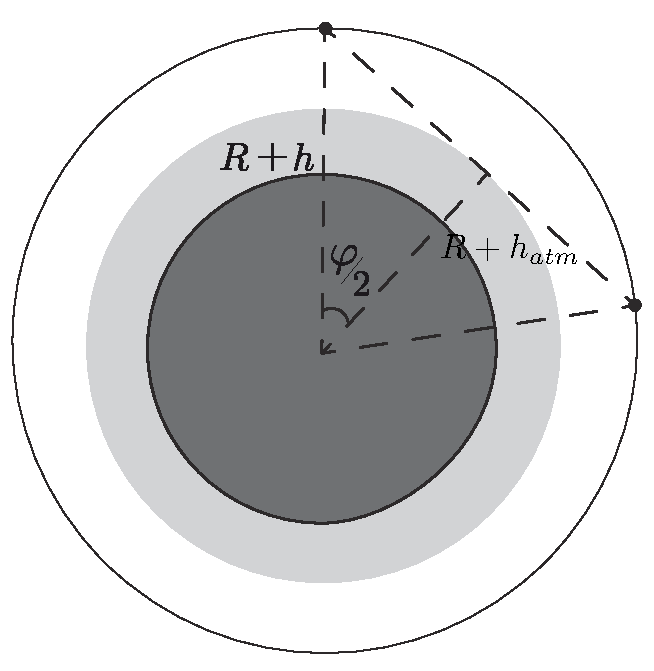
\includegraphics[scale=0.6]{./sections/3_Constellation/img/diagram.pdf}
\caption{Situation we are dealing with. In grey, the atmosphere}
\label{diagram}
\end{figure}

\paragraph{}Hence, the distance is obtained by the \textit{cosine rule}:

\begin{equation}
d = (R+h)\sqrt{2(1-cos \varphi)}
\end{equation}

\paragraph{}The results of applying this simple equations are shown in the following figure:
\begin{figure}[H]
\centering
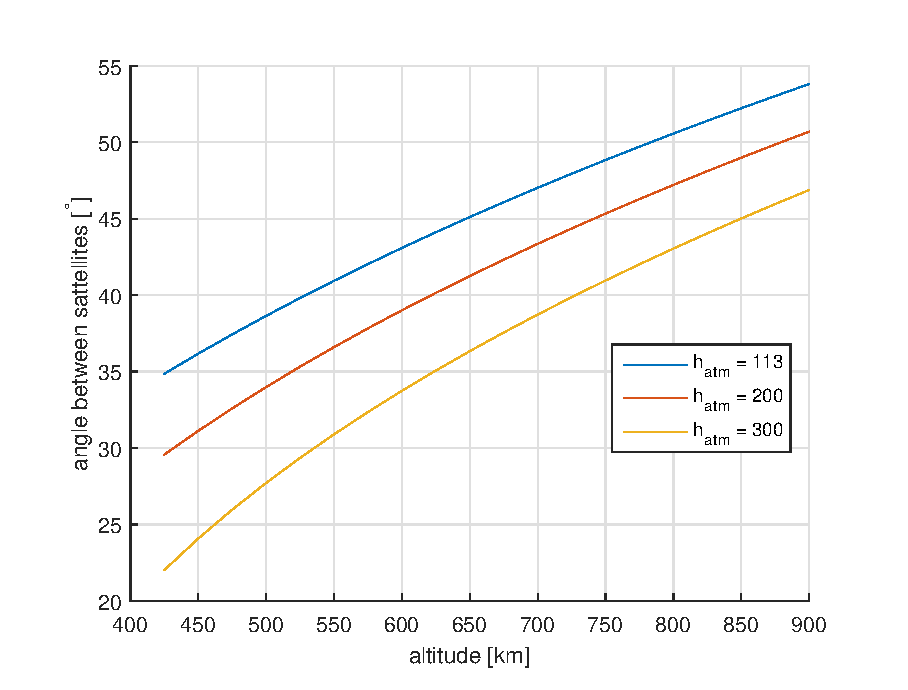
\includegraphics[scale=0.8]{./sections/3_Constellation/img/grafic.eps}
\caption{Some values of the angle between satellites for different altitudes}
\end{figure}


